\subsection{Possible applications on non periodic signals}
//es kann sein, dass ich den absatz in future work packe da er dort besser hinein passt.

This thesis has focused on periodic vibration signals rather than on signals that rise, fall or remain constant over an extended time period. Because of that it is worth investigating wether the incremental principal component analysis approach which was developed in this works can also be applied to such non periodic signals. One of the most suitable parameters for this comparison is temperature as measured on mechanical machines since temperature signals typically drift upwards or downwards slowly over time rather than following recurring structures as found in vibration signals. The pipeline was applied to the ambient temperature system failure dataset by \textcite{gokhale2012ambienttemp} which is part of the Numenta Benchmark repository which represents temterature readings from an industrial machine sensor over an extended period.
\begin{figure}[H]
\centering
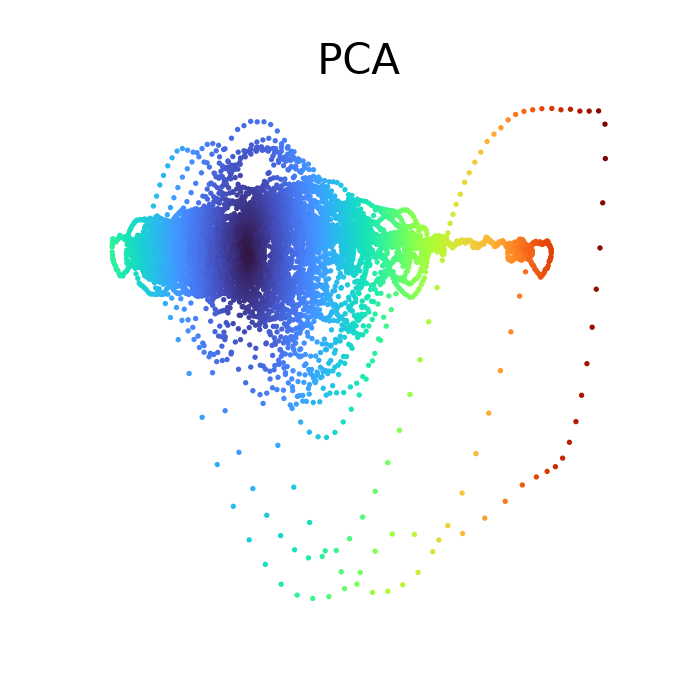
\includegraphics[width=0.5\textwidth]{figures/temperaturePlot.png}
\caption{Principle component analysis applied on non periodic data.}
\label{fig:tdeHealty}
\end{figure}
As proven in figure [n] the resulting embeddings behave clearly differently instead of forming a stable, closed shape as observed when plotting the vibration signals, the plot shows a spiral like, unwinding structure that does not repeat or represent any meaningful shape at all.